\documentclass[12pt]{article}

%     If your article includes graphics, uncomment this command.
\usepackage{graphicx}
\usepackage{times}
\usepackage[left=2.54cm, right=2.54cm, top=2.54cm]{geometry}


%    Absolute value notation
\newcommand{\abs}[1]{\lvert#1\rvert}
\newcommand{\ceil}[1]{\lceil#1\rceil}

%    Blank box placeholder for figures (to avoid requiring any
%    particular graphics capabilities for printing this document).
\newcommand{\blankbox}[2]{%
  \parbox{\columnwidth}{\centering
%    Set fboxsep to 0 so that the actual size of the box will match the
%    given measurements more closely.
    \setlength{\fboxsep}{0pt}%
    \fbox{\raisebox{0pt}[#2]{\hspace{#1}}}%
  }%
}
\begin{document}

\hspace*{\fill} Rebecca Jackson
\\
\begin{center}
\huge
\textbf{Week 8 Assignment}
\end{center}
\normalsize

\section*{Question 1}
  \begin{itemize}
    \item A one 6-sided die is rolled once, what is the probability of getting a 3 given you know the number is odd?
    \begin{itemize}
      \item There are three odd values on a 6-sided die. Thus $P(3|odd)=\frac{1}{3}$
    \end{itemize}
    \item What is the probability that the total of two dice will be greater than 8, given that the first die is a 5?
    \begin{itemize}
      \item $P(D_1+D_2 > 8 | D_1=5)= \frac{P((D_1+D_2 > 8) \cap P(D_1=5|D_1+D_2 > 8))}{P(D_1=5)}= \frac{(\frac{10}{36}) \cdot (\frac{5}{10})}{\frac{1}{6}}=\frac{5}{6}=.833$
    \end{itemize}
  \end{itemize}
\section*{Question 2}
A CSU Professor surveyed 100 high school students on which course they would most like to study at CSU after leaving high school. This two-way table displays data for the sample of students who responded to the survey.
\\

\begin{tabular}{|c|c|c|c|}
  \hline
  Course & Male & Female & Total\\
  \hline
  CompSc & 26 & 12 & 38 \\
  \hline
  Physics & 12 & 32 & 44\\
  \hline
  Biology & 10 & 8 & 18\\
  \hline
  \textbf{TOTAL} & 48 & 52 & 100 \\
  \hline
\end{tabular}
\\
  \begin{itemize}
    \item A student is chosen at random. Find the probability that the student chose to study CompSc.
    \begin{itemize}
      \item $P(CompSc)= \frac{38}{100}=.38$
    \end{itemize}
    \item Find the probability of that the student is a male.
    \begin{itemize}
      \item $P(Male)= \frac{48}{100}=.48$
    \end{itemize}
    \item Find the probability of that the student is a female.
    \begin{itemize}
      \item $P(Female)= \frac{52}{100}=.52$
    \end{itemize}
    \item Find the probability that the student is a male given that he chose to study CompSc.
    \begin{itemize}
      \item $P(Male|CompSc)= \frac{P(Male \cap CompSc)}{P(CompSc)}=\frac{\frac{26}{100}}{\frac{38}{100}}=\frac{26}{38}=.684$
    \end{itemize}
    \item Find the probability that the student is a female given that she chose to study CompSc.
    \begin{itemize}
      \item $P(Female|CompSc)= \frac{P(Female \cap CompSc)}{P(CompSc)}=\frac{\frac{12}{100}}{\frac{38}{100}}=\frac{12}{38}=.333$
    \end{itemize}
    \item Find the probability that the student chose to study CompSc, given that the student was male.
    \begin{itemize}
      \item $P(CompSc|Female)= \frac{P(CompSC \cap Female)}{P(Female)}=\frac{\frac{12}{100}}{\frac{52}{100}}=\frac{12}{52}=.231$
    \end{itemize}
    \item Find the probability that the student chose to study CompSc, given the student was female.
    \begin{itemize}
      \item $P(CompSc|Male)= \frac{P(CompSC \cap Male)}{P(Male)}=\frac{\frac{26}{100}}{\frac{48}{100}}=\frac{26}{48}=.542$
    \end{itemize}
  \end{itemize}
\section*{Question 3}
\subsection*{Question 3a}
A student has 80\% chance of getting to class on time if his alarm rings but only a 30\% if it does not ring. The alarm rings 90\% of the time.
  \begin{itemize}
    \item What is the probability of the student getting to class on time?
    \begin{itemize}
      \item $P(class\; on\; time)= (.8 \cdot .9)+(.3 \cdot .1)=.72+.03=.75=75\%$
    \end{itemize}
    \item The student is late for class today. What is the probability that his alarm did not work this morning?
    \begin{itemize}
      \item $P(no\;alarm|late)=\frac{P(no\;alarm\cap late)}{P(late)}=\frac{P(late|no\;alarm)\cdot P(no\;ring)}{P(late)}= \frac{.7\cdot .1}{.25}=\frac{.07}{.25}=.28=28\%$
    \end{itemize}
  \end{itemize}
\subsection*{Question 3b}
A football team wins half of its games. When the star plays the team wins 70\% of its games, but the star only plays 60\% of the games.
\begin{itemize}
  \item In what proportion of games does the team win and the star play?
  \begin{itemize}
    \item $P(win \cap star)=P(win|star)\cdot P(star)= .7 \cdot .6= .42$
    \item Out of every 100 games, there will be 42 where the team wins and the star plays.
  \end{itemize}
  \item If the team wins, what is the probability that the star played?
  \begin{itemize}
    \item $P(star|win)=\frac{P(win \cap star)}{P(win)}=\frac{.42}{.5}=.84$
  \end{itemize}
  \item Would you say that the event ``the team wins'' is independent of the event ``the star plays''? Why?
  \begin{itemize}
    \item I would say that the team wins is not independent of the star plays. This is due to the fact that $P(win \cap star) \neq P(win)\cdot P(star)$.
  \end{itemize}
\end{itemize}
\subsection*{Question 4}
\begin{itemize}
  \item The Code \\
  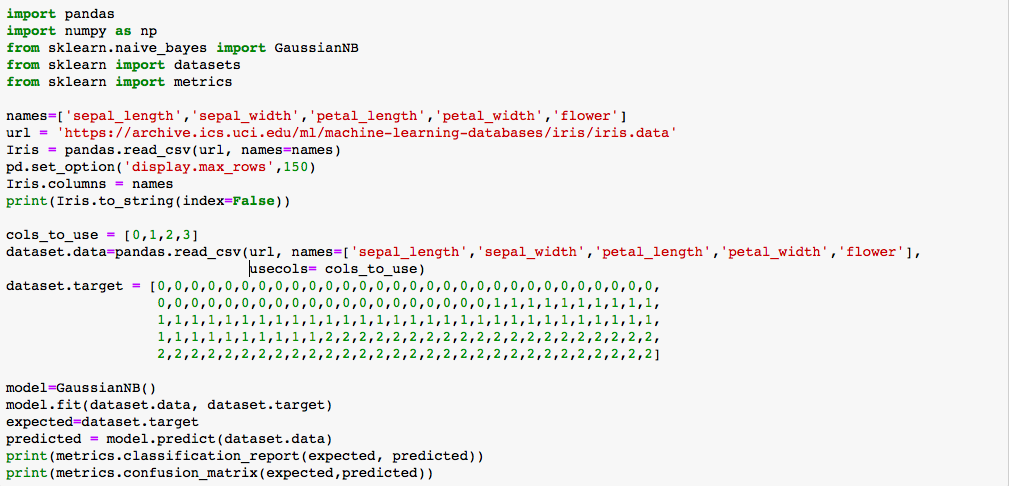
\includegraphics[width=0.75\linewidth]{code.png}
  \item The Probabilities \\
  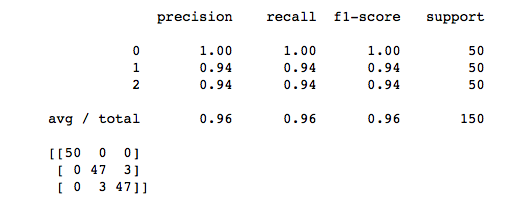
\includegraphics[width=0.75\linewidth]{probabilites.png}
  \clearpage
  \item Printing the Data \\
  
\includegraphics[width=0.3\linewidth]{data_print.jpg}
\end{itemize}
\end{document}
